%%「論文」,「レター」,「レター(C分冊)」,「技術研究報告」などのテンプレート
%% v3.4 [2023/09/12]
%% 1. 「論文」
% \documentclass[paper]{ieicej}
\documentclass[technicalreport]{ieicej}

% \documentclass[invited]{ieicej}% 招待論文
%\documentclass[survey]{ieicej}% サーベイ論文
%\documentclass[comment]{ieicej}% 解説論文
\usepackage[dvipdfmx]{graphicx,xcolor}
%%\usepackage[dvips]{graphicx}
\usepackage[fleqn]{amsmath}
%\usepackage{amsthm}
\usepackage{newtxtext}% 英数字フォントの設定を変更しないでください
\usepackage[varg]{newtxmath}% % 英数字フォントの設定を変更しないでください
%\usepackage{amssymb}
%\usepackage{bm}
\usepackage{listings,jvlisting} %日本語のコメントアウトをする場合jvlisting(もしくはjlisting)が必要
%ここからソースコードの表示に関する設定
\lstset{
  basicstyle={\ttfamily},
  identifierstyle={\small},
  commentstyle={\smallitshape},
  keywordstyle={\small\bfseries},
  ndkeywordstyle={\small},
  stringstyle={\small\ttfamily},
  frame={tb},
  breaklines=true,
  columns=[l]{fullflexible},
  numbers=left,
  xrightmargin=0zw,
  xleftmargin=3zw,
  numberstyle={\scriptsize},
  stepnumber=1,
  numbersep=1zw,
  lineskip=-0.5ex,
  % extendedchars=false, % ★ 日本語の縦書き化を防止
}
\renewcommand{\lstlistingname}{プログラム}% ソースコードのキャプションの名称

\setcounter{page}{1}

\field{A}
\jtitle{状態遷移図ベースのコード生成とログ可視化機能を備えたセンサネットワーク実機検証基盤の開発}
\etitle{}
\authorlist{%
 \authorentry[24w6047a@shinshu-u.ac.jp]{辻村篤志}{Atsushi Tsujimura}{信州大学}\MembershipNumber{}
 \authorentry{小林侑生}{Yu Kobayashi}{信州大学}\MembershipNumber{}
 \authorentry{不破泰}{Yasushi Fuwa}{信州大学}\MembershipNumber{}
 \authorentry{アサノデービッド}{David Asano}{信州大学}\MembershipNumber{}
 %\authorentry{和文著者名}{英文著者名}{所属ラベル}\MembershipNumber{}
 %\authorentry[メールアドレス]{和文著者名}{英文著者名}{所属ラベル}\MembershipNumber{}
 %\authorentry{和文著者名}{英文著者名}{所属ラベル}[現在の所属ラベル]\MembershipNumber{}
}
\affiliate[Nagano]{信州大学 〒380-0928 長野県長野市若里4-17-1}
 {Shinshu University, 4--17--1 Wakasato, Nagano-shi, 
  Nagano 380--8553 Japan}
%\affiliate[所属ラベル]{和文所属}{英文所属}
%\paffiliate\[]{}
%\paffiliate[現在の所属ラベル]{和文所属}
\jalcdoi{???????????}% ← このままにしておいてください

\begin{document}
\begin{abstract}
%和文あらまし 500字以内
センサネットワークの開発は幅広い専門知識と多大な工数を要する。先行研究では、センサネットワークの動作を表す状態遷移図からコードを生成し、汎用ハード上で動作する環境が構築されてきた。本研究ではその環境を拡張し、その上で実用的な無線通信プロトコルを実装・検証した。その過程で汎用ハード上でのプロトコルの動作が確認しづらいことを課題として認識し、デバッグ用ログ出力とそれを可視化・ステップ実行できる環境を開発しデバッグ効率の向上を図った。
\end{abstract}
\begin{keyword}
%和文キーワード 4〜5語
無線センサーネットワーク、無線通信プロトコル、状態遷移図、コード生成、ログ可視化
\end{keyword}

\begin{eabstract}
%英文アブストラクト 100 words
The development of sensor networks requires extensive expertise and significant effort. Previous research has generated code from state transition diagrams representing the behavior of sensor networks, establishing an environment that operates on general-purpose hardware. This study expands that environment and implements and verifies practical wireless communication protocols. During this process, we recognized the difficulty in confirming the operation of protocols on general-purpose hardware as a challenge and developed an environment for debugging log output and visualizing and step-executing it to improve debugging efficiency.
\end{eabstract}

\begin{ekeyword}
%英文キーワード
wireless sensor networks, wireless communication protocols, state transition diagrams, code generation, log visualization
\end{ekeyword}
\maketitle

% _/_/_/_/_/_/_/_/_/_/_/_/_/_/_/_/_/_/_ 1章 /_/_/_/_/_/_/_/_/_/_/_/_/_/_/_/_/_/_/_/_/_/_/_/_/_/_/_/_/_/_/
\section{はじめに}
\subsection{背景}
近年、無線センサネットワーク(Wireless Sensor Network:WSN)は、環境モニタリングやスマートシティ、インフラ監視、農業、ヘルスケアなど、さまざまな分野での応用が期待されている。実際、WSNを含むIoTデバイスの数は2020年時点で約130億台に達し、年率20%で増加しており、2025年には300億台弱に到達すると予測されている\cite{jst2022}. また、MDPIの報告によれば、WSNノードの数は2012年の約4.5億台から2022年には約20億台へと拡大しており\cite{mdpi2021}、その研究および実用の両面での発展が顕著である。  
しかし、これらのシステムを構築するためには、複雑な通信プロトコル設計やデータ処理アルゴリズムの実装が求められ、開発者には高度な専門知識と多大な工数が必要となる。そのため、システム開発の効率化や開発者支援を目的とした研究が進められている。
\vskip\baselineskip

\subsection{従来研究}
従来研究では、無線通信プロトコルの状態遷移図から自動生成したプログラムを汎用ハード上で動作させ、CSMAおよびTDMAベースのMACプロトコルを実機で実装・検証できる環境が構築されていた(旭ら)。このシステムにより基本的な通信プロトコルの動作検証が可能となったが、デバッグ方法はシリアルコンソールへのログ出力に依存しており、通信処理が高速に進むため逐次的な状態遷移を追跡することが難しかった。その結果、異常動作の原因を把握しづらく、開発効率や教育的利用の観点では十分でない点が課題として残されていた。

\vskip\baselineskip
\subsection{目的}
本研究の目的は、従来研究で課題となっていたデバッグ効率の低さを改善し、実機でのプロトコル検証をより効果的に行える環境を実現することである。そのために、状態遷移図から生成したコードの動作をログとして出力し、それを可視化・ステップ実行できる仕組みを開発した。これにより、プロトコルの動作を逐次的に把握でき、異常動作の原因究明を容易にするとともに、教育や応用実証に適した支援環境を提供することを目指す。
\vskip\baselineskip




% _/_/_/_/_/_/_/_/_/_/_/_/_/_/_/_/_/_/_ 2章 /_/_/_/_/_/_/_/_/_/_/_/_/_/_/_/_/_/_/_/_/_/_/_/_/_/_/_/_/_/_/
\section{提案システム}
\subsection{システム構成}
本研究で開発したシステムの全体構成を図\ref{fig:system-composition}に示す。本システムは、状態遷移図を入力としてC++プログラムを自動生成し、PlatformIO上でビルドを行い、汎用ハードウェア上で実行することでセンサネットワークのプロトコルの動作検証を可能とする。さらに、通信動作の状態遷移や変数値の過程をログとして記録し、ブラウザ上で状態遷移の可視化およびステップ実行を行える環境を備えている。これにより、プロトコル設計から実機検証、デバッグまでを一貫して支援することが可能となる。
\vskip\baselineskip
\begin{figure}[tb]
  \centering
  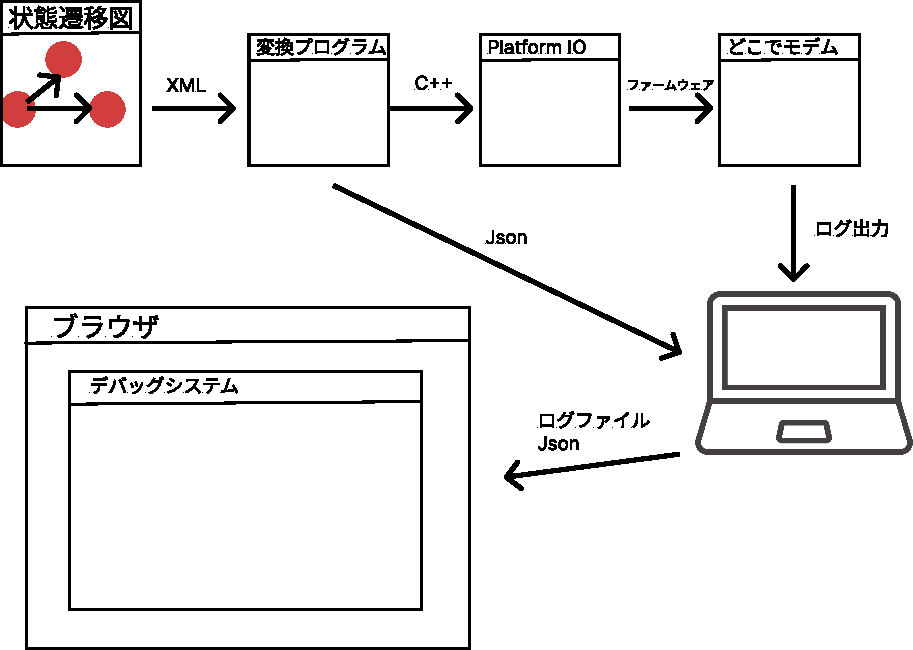
\includegraphics[width=80mm]{./images/system-composition.pdf}
  \caption{提案システムの全体構成}
  \ecaption{Block diagram of the proposed system.}
  \label{fig:system-composition}
\end{figure}


\subsection{ファームウェア生成部}
ファームウェア生成部では,無線通信プロトコルの動作をAstah Professional上の状態遷移図として設計し,XML形式で出力する。次に,変換プログラム(Python)を用いて状態遷移図のXMLをC++プログラムへ変換し,PlatformIO環境でビルドすることでファームウェアを生成する。このファームウェアは2.3節で述べる汎用ハードウェア上で実行される。

先行研究(小林ら\cite{kobayashi2023})では,状態遷移図の各要素(通信状態・遷移・初期値設定・処理内容など)をXMLファイルから抽出し,それぞれをリスト化したうえで,通信状態間の関係を解析し,C++の`switch-case`構造に変換するアルゴリズムが実装されている。本研究におけるファームウェア生成部は,この変換処理を利用しており,状態遷移図で設計されたプロトコル仕様を汎用ハードウェア上で動作するプログラムとして自動生成するものである。

図\ref{fig:state-machine}に状態遷移図の例を,プログラム\ref{converted-code}に変換後のC++コードを示す。状態遷移図で定義された「待機(LISTEN)」「受信(RECEIVE)」「送信(TRANSMIT)」の各状態と遷移関係が,`switch-case`構造によって対応づけられており,設計段階の論理構造がソースコードとして正しく反映されていることが確認できる。

\vskip\baselineskip
\begin{figure}[tb]
  \centering
  \includegraphics[width=60mm]{./images/state-machine-image.png}
  \caption{状態遷移図の例}
  \ecaption{State transition diagram.}
  \label{fig:state-machine}
\end{figure}

\begin{figure}
\begin{lstlisting}[caption={変換されたC++プログラム}, label=converted-code]
typedef enum { LISTEN, RECEIVE, TRANSMIT } NodeState;

void protocol_main() {
  switch (state) {
    case LISTEN:   updateState(RECEIVE);   break;
    case RECEIVE:  updateState(TRANSMIT);  break;
    case TRANSMIT: updateState(LISTEN);    break;
  }
}
\end{lstlisting}
\end{figure}
\vskip\baselineskip




\subsection{実行環境(ハードウェア)}
次に,実行環境について述べる。本システムでは,SAMD21マイコンを搭載した無線モデム(株式会社サーキットデザイン製どこでモデム)を用い,生成したファームウェアを書き込み実行する。このモデムは429 MHz帯で動作する汎用的な無線モデムであり,技術基準適合証明を取得しているため,実際に電波を送受信しながら通信プロトコルの検証を行うことができる。また,429 MHz帯は中山間地域において回折性能に優れており,低消費電力で長距離通信が可能なLPWA(Low Power Wide Area)通信に適している。この特性を活かすことで,将来的には登山者見守りシステムなどへの応用も期待できる。さらに,本モデムはマイコンと通信モジュールが一体化しているため,外部配線や追加ハードウェアを必要とせず,開発や実験環境の構築を容易に行うことが可能である。加えて,GPSモジュールを併用することで,位置情報の取得および1PPS信号による高精度な時刻同期を実現し,複数ノード間での無線通信プロトコルの正確な動作検証を可能としている。
\vskip\baselineskip
\begin{figure}[tb]
  \centering
  \includegraphics[width=60mm]{./images/devices.jpg}
  \caption{どこでモデム(左)とGPSモジュール(右)}
  \ecaption{Block diagram of the proposed system.}
  \label{fig:system}
\end{figure}

\subsection{デバッグシステム部}
本節では,通信プロトコルの動作を可視化し,逐次的なデバッグを可能とするデバッグシステムについて述べる。提案システムは,ファームウェアが出力するログを入力として,ブラウザ上で状態遷移の再現と変数追跡を行う仕組みを備える。これにより,開発者は通信の挙動を視覚的に理解でき,異常箇所の切り分けを効率化できる。
\vskip\baselineskip

\subsubsection{UI構成}
図\ref{fig:viewer-ui}に可視化画面の構成を示す。画面上部にログファイル(テキスト)および状態遷移図ファイル(JSON)のアップロード領域を配置し,中央にステップ実行用のボタン群(次,前,最初に戻る)とスライダを設ける。下部は「変数追跡」「ログ表示」「状態遷移図描画」の3領域で構成し,処理の流れと内部状態を統合的に把握できる設計とした。
% UIの画像
\begin{figure}[tb]
  \centering
  \includegraphics[width=80mm]{./images/viewer_ui.png}
  \caption{ログ可視化・ステップ実行環境のUI}
  \ecaption{User interface of the log visualization and step execution environment.}
  \label{fig:viewer-ui}
\end{figure}
\vskip\baselineskip

\subsubsection{ログ出力形式}
各状態遷移および変数変化は,識別可能な最小単位で逐次ログ化する。状態は
\begin{verbatim}
STATE:LISTEN
STATE:RECEIVE
\end{verbatim}
のように1行1状態で出力し,変数は
\begin{verbatim}
[VAR:current_slot=3]
[VAR:has_own_slot=true]
\end{verbatim}
のように \verb|[VAR:<name>=<value>]| 形式で出力する。値は数値・文字列の双方を許容し,可視化側で時系列に統合して解析する。単純で曖昧さの少ない表記とすることで,正規表現に基づく軽量なパーサで高速に処理できる。

さらに,ログ出力の形式にばらつきが生じないよう,C++のマクロを用いてログ出力関数を定義している。このマクロは,変数名と値を自動的に取得して \verb|[VAR:<name>=<value>]| 形式で出力するため,開発者は変数名を明示する必要がない。例えば,ユーザは \verb|PRINT_VAR_LOG(変数)| のように記述するだけで統一フォーマットのログを生成できる。この仕組みにより,全ての出力が一定形式で記録され,可視化システム側で確実に解析可能となる。
\vskip\baselineskip


\subsubsection{可視化・再現機構}
本システムでは,記録されたログファイルと,状態遷移図の構造を記述したJSONファイルをもとに状態遷移を再現する。具体的には,JSONファイルから状態名および遷移関係を抽出し,それらをMermaid.jsのフォーマットへ変換して描画処理に渡す。ログの進行に合わせて該当ノードをハイライトすることで,通信処理の時系列的な動作を視覚的に確認できる。

Mermaid.jsは,テキストベースでフローチャートや状態遷移図を描画できる軽量なJavaScriptライブラリであり,HTML上での埋め込みや動的描画に適している。本研究では,ブラウザ環境のみで動作し,追加ソフトを必要としない点,および構文が簡潔で自動生成との親和性が高い点から採用した。これにより,状態遷移図を表すJSONデータから自動的にMermaid記法を生成し,\verb|stateDiagram-v2|形式で描画することで,設計段階の論理構造をそのままの形で可視化できる。

なお,可視化に用いるJSONファイルは,2.2節で述べたファームウェア生成部と同一のPythonプログラムによって自動的に生成される。Astah Professionalから出力された状態遷移図のXMLを解析し,C++コード生成と同時に,状態遷移関係をJSON形式で出力している。この仕組みにより,設計情報と可視化データの不整合を防ぎ,設計・実装・可視化の一貫性を確保している。
\vskip\baselineskip

図\ref{fig:json-structure}に生成されるJSONファイルの例を示す。このJSONは,状態リストと遷移リストの2つの要素で構成されており,状態名およびそれらを結ぶ遷移関係を保持する。

\begin{figure}[tb]
\begin{lstlisting}[caption={状態遷移図を表すJSONファイルの例},label=json-structure]
{
  "states": [
    "LISTEN",
    "RECEIVE",
    "TRANSMIT",
    "WAIT_ACK"
    ],
  "transitions": [
    {"from": "LISTEN", "to": "RECEIVE"},
    {"from": "RECEIVE", "to": "TRANSMIT"},
    {"from": "TRANSMIT", "to": "WAIT_ACK"},
    {"from": "WAIT_ACK", "to": "LISTEN"}
    ]
}
\end{lstlisting}
\end{figure}

ここで,\texttt{states}配列は通信状態の一覧を表し,\texttt{transitions}配列は状態間の遷移関係を示す。\texttt{from}および\texttt{to}がそれぞれ遷移元と遷移先の状態を表している。このデータ構造をもとにMermaid.js形式のテキストを自動生成し,ブラウザ上で状態遷移図を描画している。

変換後のMermaid.jsフォーマットをプログラムnに示す。
\begin{figure}[tb]
  \begin{lstlisting}[caption={生成されたMermaid.jsフォーマットの例},label=mermaid-example]
stateDiagram-v2
[*] --> LISTEN
LISTEN --> RECEIVE
  RECEIVE --> TRANSMIT
  TRANSMIT --> WAIT_ACK
  WAIT_ACK --> LISTEN
\end{lstlisting}
\end{figure}

このように,シンプルなJSON構造を中間表現として用いることで,XMLから生成された設計情報を軽量に扱うことができ,状態遷移構造の可視化を容易に実現している。
\vskip\baselineskip


\subsubsection{ステップ実行および変数追跡}
本システムでは,通信プロトコルの動作を1ステップ(1状態遷移)単位で再現できるステップ実行機能を備えている。画面上部に配置された「次のステップ」「前のステップ」「最初に戻る」ボタンにより,状態遷移を順方向または逆方向に逐次移動でき,通信処理の流れを段階的に確認することが可能である。さらに,スライダを用いることで任意のステップ位置へ直接移動でき,興味のある箇所を即座に調査できる柔軟な操作性を実現している。

状態遷移の再生にあたっては,ログの各行を1状態単位として扱い,時系列に沿って状態情報を更新する。ログ再生に合わせて,中央のログ表示領域,右側の状態遷移図,および左側の変数表示領域が同期して更新されるよう設計されている。これにより,ある状態における変数値の変化や,その状態から次への遷移を同時に確認できる。特に,状態遷移図上では現在の状態ノードがハイライト表示され,通信動作の進行位置を視覚的に把握しやすい構成となっている。

変数追跡機能では,ログ出力された任意の変数を選択し,その値の変化を時系列に追跡できる。追跡対象の変数は複数追加可能であり,状態変化とあわせて観察することで,通信プロトコルの内部状態を多角的に解析できる。これらの機能により,特定条件下での変数の変化や分岐挙動を直感的に検証でき,デバッグおよび設計検証の効率向上に寄与する。

% ステップ実行中の画面(ラベル名を重複させない)
\begin{figure}[tb]
  \centering
  \includegraphics[width=80mm]{./images/viewer_ui.png}
  \caption{ステップ実行時の状態ハイライト例}
  \ecaption{Example of state highlighting during step execution.}
  \label{fig:viewer-ui-step}
\end{figure}
\vskip\baselineskip

\subsubsection{リアルタイム可視化}
本システムの拡張として,実機で動作するファームウェアのログをリアルタイムに取得・可視化する機能を試作した。図\ref{fig:realtime-structure}にその構成を示す。

デバイス上で動作するファームウェアは,通信動作に応じて状態遷移ログをシリアルポートへ逐次出力する。Pythonスクリプトがこのシリアルポートを常時監視し,取得したログデータをMQTT(Message Queuing Telemetry Transport)プロトコルを介してバックエンドサーバへ送信する。MQTTは軽量なPub/Sub型通信方式であり,組込みデバイスとサーバ間のリアルタイム通信に適している。

バックエンドでは,Node.js上で動作するサーバがMQTTブローカーからログデータを受信し,Socket.IOを用いてブラウザと双方向通信を行う。これにより,取得された状態遷移情報はフロントエンドへ逐次転送され,ブラウザ上のMermaid.jsによる状態遷移図に即時反映される。通信遅延は数百ミリ秒程度に抑えられ,状態の変化をほぼリアルタイムに確認できることを確認した。

この構成により,従来の「ログ取得→解析→可視化」といった事後的なデバッグ手法に対し,動作中のシステム挙動を即時に観測できる「実時間デバッグ」が可能となった。これにより,通信プロトコルの動作確認やノード間同期の評価を効率化できるだけでなく,将来的には実験中の異常検知や教育用デモ環境への応用も期待される。

一方で,状態遷移の周期が非常に短いプロトコルや高速に状態が変化するシステムにおいては,描画更新が処理速度に追従できず,視認性が低下する場合がある。このため,本機能は主に周期の長い通信プロトコルや教育目的の可視化において有効であり,高速プロトコルの解析にはログ記録・再生型の可視化機構(2.4節)を併用することが望ましい。


% リアルタイムのシステム設計図、検討
% \begin{figure}[tb]
%   \centering
%   \includegraphics[width=80mm]{./images/realtime_structure.pdf}
%   \caption{リアルタイム可視化機能の構成}
%   \ecaption{System structure of the real-time visualization function.}
%   \label{fig:realtime-structure}
% \end{figure}
\vskip\baselineskip


% _/_/_/_/_/_/_/_/_/_/_/_/_/_/_/_/_/_/_ 3章 /_/_/_/_/_/_/_/_/_/_/_/_/_/_/_/_/_/_/_/_/_/_/_/_/_/_/_/_/_/_/
\section{プロトコル実装と評価}

\subsection{プロトコルの実装}
本節では,状態遷移図から自動生成されたファームウェアを用いて実装した無線通信プロトコルについて述べる。本プロトコルは,園田ら\cite{sonoda2021}によるCSMA/TDMA混在型プロトコルを参考として設計したものであり,TDMAによるスロット分割を基本構造としつつ,各端末が自律的に送信スロットを決定する点に特徴を持つ。

通信は,中継器(集約機)1台と複数の端末ノードとの間で行われる。通信フレームは複数のスロットで構成され,最初のスロットにおいて中継器が全端末に対してスロットの占有状況を通知する。各端末はこの情報をもとに,自ノードの送信スロット候補を自律的に選択する。選択したスロットが空いていると判断した端末は,そのスロットにおいてリクエストパケットを送信し,中継器からACK応答を受信した時点でスロットを確定・占有する。

一方で,ACKが返ってこなかった場合や他ノードとの競合が発生した場合は,再びスロット情報の受信状態に戻り,次フレームで再試行を行う。このように,各端末が占有状況に基づいて分散的にスロットを決定することで,集中制御を必要とせずに動的なスロット割り当てを実現している。

図\ref{fig:protocol-state-machine}に本プロトコルの主要な状態遷移図を示す。本図は,実装上の例外処理や再送制御を省略し,主要な通信経路のみを示している。初期状態\texttt{IDLE}から開始し,スロット情報の受信(\texttt{RECEIVE\_SLOT\_INFO}),スロット候補の決定(\texttt{CHECK\_SLOT}),リクエスト送信(\texttt{TRANSMIT}),ACK待機(\texttt{WAIT\_ACK}),スロット確定(\texttt{UPDATE\_SLOT})を経て,再び\texttt{IDLE}に戻るサイクル構造を有する。

\begin{figure}[tb]
  \centering
  \includegraphics[width=80mm]{./images/protocol-state-machine3.png}
  \caption{開発したCSMA/TDMAベース無線通信プロトコルの状態遷移図(主要経路のみ)}
  \ecaption{State transition diagram of the developed CSMA/TDMA-based wireless communication protocol (simplified main flow).}
  \label{fig:protocol-state-machine}
\end{figure}


\subsection{実験}
提案システムの有効性を確認するため,開発したCSMA/TDMAベースのプロトコルを2.2節で述べた汎用ハードウェアに適用し,実機通信実験を行った。図\ref{fig:system-composition}に示す構成を用い,中継器(集約機)1台および端末ノード3台で通信を行った。各ノードにはSAMD21マイコンを搭載した無線モデムを接続し,PlatformIO環境で自動生成されたファームウェアを書き込んで動作させた。

実験では,ノード間でスロット割当からデータ送信・ACK応答までの一連の通信を実行し,状態遷移ログをシリアルポート経由で取得した。ログには各状態遷移および変数値の変化が逐次出力され,これを提案システムの可視化ツールに読み込むことで,通信動作の再現および解析を行った。

評価の観点として,以下の4点を設定した。
\begin{enumerate}
  \item \textbf{状態遷移追跡の正確性}: 通信動作中の状態変化をログから忠実に再現できるか。
  \item \textbf{デバッグ効率の向上}: 異常動作発生時に,原因箇所を迅速に特定できるか。
  \item \textbf{開発効率の向上}: 状態遷移図の修正から再生成・再実装までの手戻りを軽減できるか。
  \item \textbf{ログ可視化の有用性}: 状態遷移図上で動作過程を視覚的に理解できるか。
\end{enumerate}

これらの検証により,提案システムが通信動作の把握と異常検出を容易にし,デバッグ・開発両面での作業効率を向上させることを確認した。

\subsection{評価}
提案システムの有効性を,従来のコンソール出力によるデバッグ手法と比較して評価した。従来手法では,シリアルモニタに出力されるログを目視で追跡し,異常動作の原因を特定していた。しかし,通信処理はミリ秒単位で進行するため,出力ログの順序やタイミングのずれから状態間の関係を正確に把握することが困難であった。特に,複数の変数が同時に変化する場面では因果関係の分析が煩雑になり,開発者の負担が大きかった。

一方,提案システムでは,ログを自動解析し,状態遷移図上に反映することで通信動作を直感的に把握できる。図\ref{fig:viewer-ui}に示すように,現在の状態がハイライト表示され,対応するログ行および変数値が同期して更新される。この視覚的同期表示により,特定時点での状態と内部変数の関係を明確に追跡できる。

さらに,ステップ実行機能を備えることで,通信動作を1状態単位で前後に移動できる。「次のステップ」「前のステップ」「最初に戻る」ボタンの操作により,異常発生箇所の直前・直後を逐次確認でき,原因特定の時間を大幅に短縮できた。また,スライダーを用いて任意のステップにジャンプできるため,ログの中で特定区間のみを重点的に調査することも可能である。

加えて,変数追跡機能により,複数の変数を同時に監視しながら状態遷移を確認できる。例えば,スロット番号(\texttt{current\_slot})とACKフラグ(\texttt{ack})を同時に追跡することで,ACK未受信時にどのスロットで異常が発生したかを容易に特定できた。従来のコンソール出力では,変数の変化を時系列で突き合わせる必要があったが,提案システムでは視覚的に統合されており,動作過程を体系的に理解できる。

これらの評価結果より,提案システムは従来のログベースデバッグに比べて,
\begin{itemize}
  \item 状態遷移の追跡が容易で,通信処理の因果関係を直感的に把握できる。
  \item ステップ実行機能により,異常動作の原因特定時間を大幅に短縮できる。
  \item 複数変数を同時に可視化でき,通信内部の動作理解が促進される。
\end{itemize}
ことを確認した。特に,状態遷移・変数・ログを統合的に扱える点は,デバッグ効率の向上だけでなく,教育的利用や通信プロトコル設計演習にも有用であると考えられる。

図\ref{fig:old-debug}に従来のコンソールベースのデバッグ方法を,図\ref{fig:viewer-ui}に提案システムによるログ可視化・ステップ実行環境を示す。提案システムにより,通信動作の全体像を俯瞰しながら,詳細な内部状態を逐次的に追跡できる環境が実現された。

\begin{figure}[tb]
  \centering
  \includegraphics[width=50mm]{./images/old_debug.png}
  \caption{従来のコンソール出力によるデバッグ方法}
  \ecaption{Example of the traditional console-based debugging method.}
  \label{fig:old-debug}
\end{figure}

\begin{figure}[tb]
  \centering
  \includegraphics[width=80mm]{./images/step_3.png}
  \caption{提案システムによるログ可視化・ステップ実行環境}
  \ecaption{Log visualization and step execution environment of the proposed system.}
  \label{fig:viewer-ui}
\end{figure}
\vskip\baselineskip

% _/_/_/_/_/_/_/_/_/_/_/_/_/_/_/_/_/_/_ 4章 /_/_/_/_/_/_/_/_/_/_/_/_/_/_/_/_/_/_/_/_/_/_/_/_/_/_/_/_/_/_/
\section{考察}
本研究で開発したログ可視化システムにより,通信プロトコルの動作過程を逐次的に追跡できることを確認した。これにより,従来のコンソール出力のみに依存したデバッグ手法に比べて,通信動作を直感的かつ体系的に理解することが可能となった。特に,状態遷移図上で現在の状態や変数の変化を視覚的に把握できる点は,デバッグ効率の向上に大きく寄与する。

従来手法では,高速で進行する通信処理の挙動を逐一確認することが困難であり,異常動作の再現や原因特定に多くの時間を要していた。本研究の可視化環境では,ステップ実行機能により状態遷移を一段階ずつ再現できるため,処理の流れや条件分岐を容易に追跡できる。これにより,開発者が異常箇所を迅速に特定できるだけでなく,通信アルゴリズムの学習や設計意図の共有にも有効である。

また,開発した環境は教育的利用や共同研究にも有用であると考えられる。例えば,状態遷移図を教材として利用する際に,図上で通信動作を再現できることは,通信プロトコルの理解促進に寄与する。さらに,複数の開発者がログを共有しながら解析を行うことで,チーム開発時のコミュニケーション効率の向上も期待できる。

一方で,現時点のシステムにはいくつかの課題が残る。第一に,リアルタイム性の向上が挙げられる。現状では,ログを取得後に可視化する「事後解析型」が中心であり,実機動作中の挙動をリアルタイムで完全に再現するには至っていない。第二に,通信性能やデバッグ効率の改善効果を定量的に評価していない点である。定量的な指標に基づく評価を行うことで,提案システムの有効性をより客観的に示すことができると考えられる。第三に,ノード数の増加に伴うログ量の増大や可視化負荷への対応も今後の検討課題である。

総じて,本研究の成果は,通信プロトコルの開発・理解・教育を支援する基盤として有効であることを示唆しており,さらなる拡張によって幅広い応用が期待される。

\vskip\baselineskip


% _/_/_/_/_/_/_/_/_/_/_/_/_/_/_/_/_/_/_ 5章 /_/_/_/_/_/_/_/_/_/_/_/_/_/_/_/_/_/_/_/_/_/_/_/_/_/_/_/_/_/_/
\section{まとめおよび今後の展望}
本研究では,状態遷移図から自動生成したファームウェアを汎用ハードウェア上で実行し,無線通信プロトコルの動作を実機で検証可能とする環境を開発した。さらに,通信処理中に出力されるログを解析し,ブラウザ上で状態遷移および変数変化を可視化・ステップ実行できるデバッグ支援システムを実装した。

これにより,従来のコンソール出力によるデバッグでは困難であった逐次的な動作確認を可能とし,プロトコル動作の理解促進と開発効率の向上に寄与することを示した。また,状態遷移図を中心とした設計と可視化環境の統合により,通信プロトコルの設計・実装・評価を一貫して行える開発基盤を実現した。

今後の展望としては,以下の3点を挙げる。
\begin{enumerate}
\item \textbf{定量的評価の実施:} デバッグ時間やエラー検出効率などを指標として,提案システムの有効性を客観的に評価する。
\item \textbf{大規模ネットワークへの拡張:} ノード数を増加させた環境での通信挙動の検証や可視化負荷の軽減手法の検討を行う。
\item \textbf{リアルタイム可視化機能の強化:} MQTTやSocket通信を活用したリアルタイムデータストリーム処理により,実時間での挙動確認を可能とする。
\end{enumerate}

また,社会的応用としては,登山者見守りシステムなどへの展開や,通信教育・実習環境への導入が有望である。さらに,将来的には,センサデータの可視化や異常検知アルゴリズムの統合など,応用層への拡張も視野に入れて研究を継続していく。


\vskip2\baselineskip
%\bibliographystyle{sieicej}
%\bibliography{myrefs}
\bibliographystyle{junsrt}
\begin{thebibliography}{99}
\bibitem{jst2022} 科学技術振興機構: 「SIP IoE 年次報告書 2022」, 2022.
\bibitem{mdpi2021} M. R. Hasan et al.: "Recent Advancement of Data-Driven Models in Wireless Sensor Networks," *Technologies*, vol.9, no.4, 2021.
\bibitem{asahi} 旭健太、アサノデービッド、不破泰: "センサーネットワーク検証システムにおける遷移図を用いたMACプロトコル設計環境の開発", 信学技報, NS2023-xx, 2022.
\bibitem{kobayashi2023} 小林遼, アサノデービッド, 不破泰:
“センサーネットワーク検証システムにおける遷移図を用いたMACプロトコル設計環境の開発,”
信学技報, NS2023-xx, 2023.

\bibitem{PlatformIO}
\bibitem{circuitdesign}
\bibitem{astah}
\bibitem{mermaid}
\end{thebibliography}
\end{document}


